% !TeX spellcheck = en_GB
\section{Observations in December}
The general climate at Haukeliseter can be defined with the updated K\"oppen-Geiger climate types presented in \cite{peel_updated_2007}. Figure 8 in \cite{peel_updated_2007} shows, that Haukeliseter may lay in a transition zone and can be categorized as  ET, a polar tundra climate type (hottest month temperature T$_{hot}\ge$ \SI{0}{\celsius}) or Dfc, a cold climate without dry season and cold summers. 
\\
Haukeliseter presents a typical Norwegian climate condition. At the measurement site, frequent snow events combined with high wind speeds are observed during a six to seven month winter period. In addition a snow amount of about \SIrange{2}{3}{\m} can be expected, where \SI{50}{\percent} of the yearly precipitation is solid \citep{wolff_new_2010, wolff_measurements_2013, wolff_derivation_2015}. \\
The mean wind direction for solid precipitation is from the west with maximum wind speeds above \SI{15}{\mPs}, observed during a 10 year winter period at a nearby station \citep{wolff_new_2010, wolff_derivation_2015}. 
%%% images December observation %%%%%%%%%%%%%%%%%%%%%%%%%%%%%%%%%%%%%
% !TeX spellcheck = en_GB
\begin{figure}[t]
	\centering
    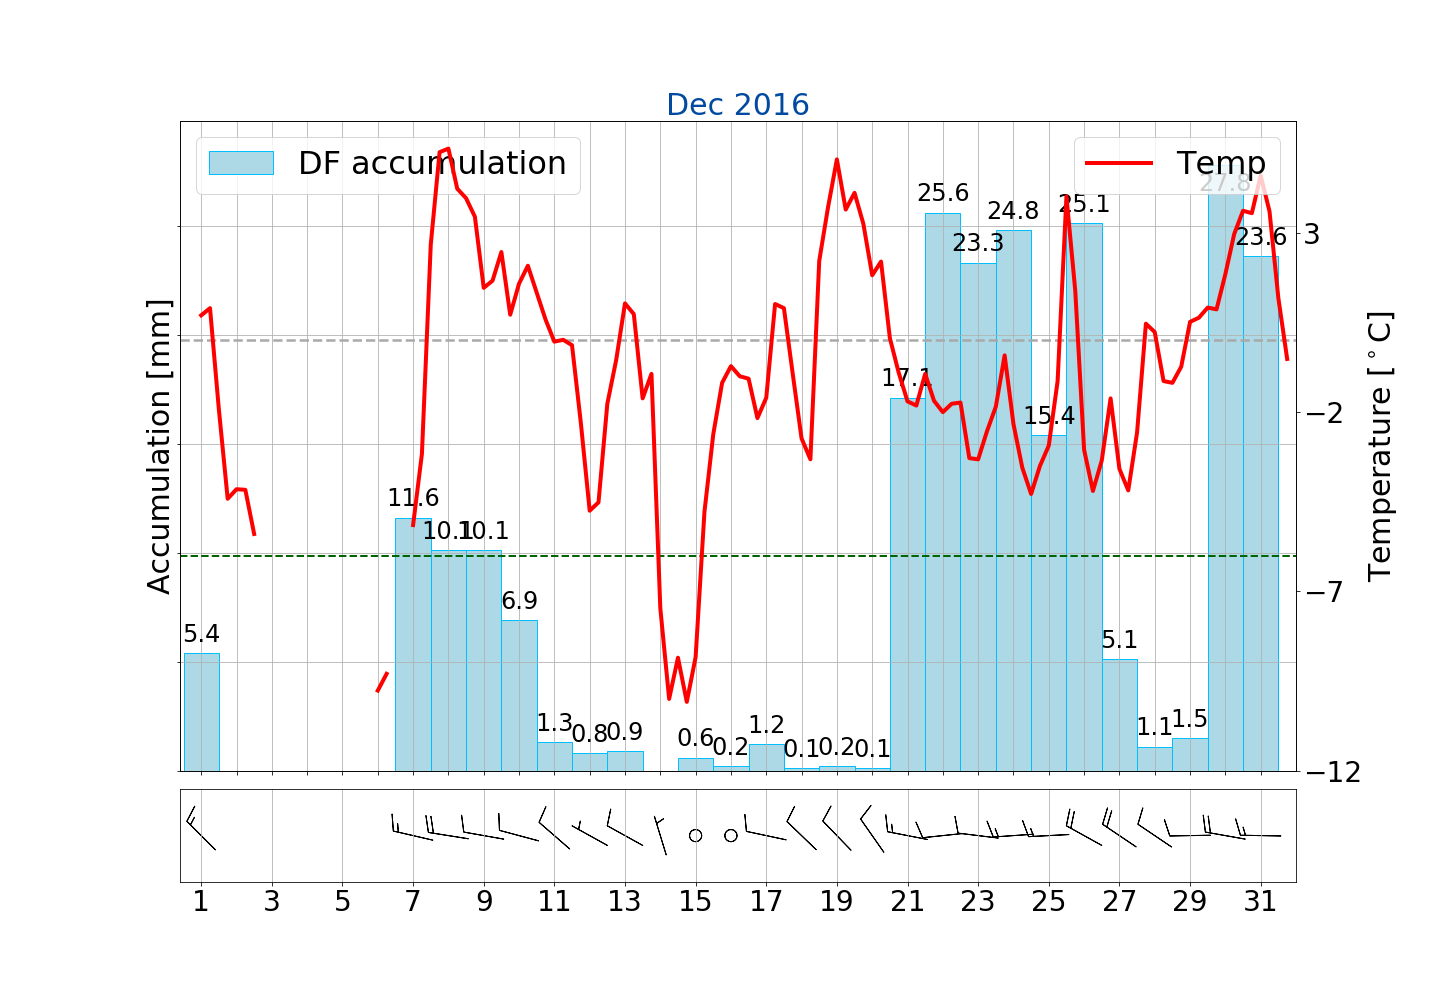
\includegraphics[trim={4.cm 3.3cm 1.5cm 3.cm},clip,
        width=0.8\textwidth]{./fig_weathermast/T_P_U_201612}
        \caption{Observations at Haukeliseter weather mast for December 2016. Daily accumulation [\SI{}{\mm}] in light blue, mean temperature every six hours (red, [\SI{}{\celsius}]), and daily maximum wind as barbs [\SI{}{\mPs}]. Gray dashed line indicates the freezing temperature. The monthly normal value is green dashed (\SI{-6.0}{\celsius}), the values are taken from \cite{eklima_norwegian_2016}. Note, that no data was available from \SIlist{2;6}{\dec}} \label{fig:DecObs}
\end{figure}
%%%%%%%%%%%%%%%%%%%%%%%%%%%%%%%%%%%%%%%%%%%%%%%%%%%%%%%%%%%%%%%%%%%%%%%%%%
\noindent As seen in \Cref{fig:DecObs} is the average December temperature \SI{-6}{\celsius} (30-yr period \numrange{1961}{1990}, value taken from \cite{eklima_norwegian_2016}).
% mean temperature in Dec was -1.1°C, climate = -6 --> dT = 4.9°C
December 2016 was warmer with an anomaly of +\SI{4.9}{\kelvin} above the climate mean. 
% total precipitation in Dec is 239.9mm, climate = 85mm --> dRR = 154.9
In 2016, the precipitation was \SI{200}{\percent} more than the climate mean. \textcolor{red}{yr.no says something different. According to them was it only \SI{76}{\percent}} 
% total precipitation during 21.-27.12. is 136.4 mm, total is 239.9mm --> 56.9%
The precipitation observed in the time period \SIrange{21}{27}{\dec} where \SI{56.9}{\percent} of the total accumulation in December 2016. Furthermore, a maximum wind of \SI{22.3}{\mPs} was observed in this period, which can be associated to a slight storm.